\begin{figure}[htbp]
	\centering
	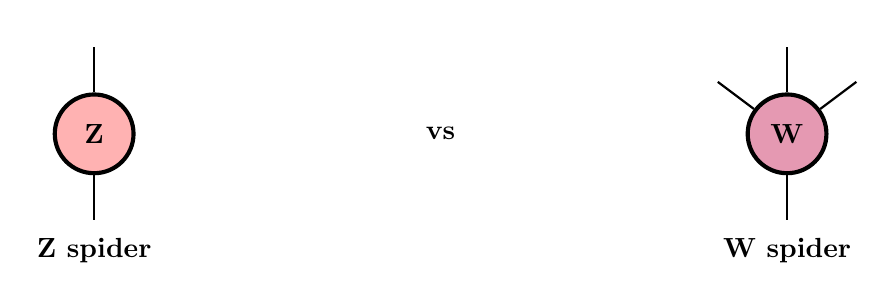
\begin{tikzpicture}[scale=1.1]
		\begin{scope}
			\node[draw, circle, fill=red!30, minimum size=1cm, line width=1.5pt] (z) at (0,0) {\textbf{Z}};
			\draw[thick] (z) -- ++(0,1) node[above] {};
			\draw[thick] (z) -- ++(0,-1) node[below] {};

			\node[below=1.2cm] at (0,0) {\textbf{Z spider}};
		\end{scope}

		\node at (4,0) {\textbf{vs}};

		\begin{scope}[xshift=8cm]
			\node[draw, circle, fill=purple!40, minimum size=1cm, line width=1.5pt] (w) at (0,0) {\textbf{W}};
			\draw[thick] (w) -- ++(0,1) node[above] {};
			\draw[thick] (w) -- ++(0.8,0.6);
			\draw[thick] (w) -- ++(-0.8,0.6);
			\draw[thick] (w) -- ++(0,-1) node[below] {};

			\node[below=1.2cm] at (0,0) {\textbf{W spider}};
		\end{scope}

	\end{tikzpicture}
	\caption{Comparison of Z and W spiders in the ZW calculus. Z spiders encode classical bits in the computational basis, while W spiders provide the primitive for genuine multipartite entanglement. This dual representation enables complete characterization of quantum states.}
	\label{fig:zw-z-vs-w}
\end{figure}
